\documentclass[a4paper]{article}
\linespread{1.6}
\usepackage{enumerate}
\usepackage{geometry}
\usepackage{setspace}
\usepackage{amsmath}
\usepackage{amssymb}
\usepackage[pdftex]{graphicx}
\usepackage{float}
\usepackage{subfigure}
\usepackage{listings}
\geometry{left=1.4cm,right=1.4cm,top=2.5cm,bottom=2.5cm}

\begin{document}
\begin{spacing}{2.0}
\begin{flushleft}\begin{huge}EEL5840 Fundamental Machine Learning   Homework 2\end{huge}\end{flushleft}
\begin{flushright}\begin{Large} Hudanyun Sheng \end{Large}\end{flushright}

\paragraph{\huge\textbf{ Question 1} } \large{Solution:\\}
	\normalsize 
	\setcounter{section}{1}
	\textbf{1.1}  $$\Sigma = \displaystyle\frac{1}{4}\left[ \begin{matrix} 5  &  \sqrt{3}\\ \sqrt{3}  &  7\end{matrix}\right] 
													 = \left[ \begin{matrix} 5/4  &  \sqrt{3}/4\\  \sqrt{3}/4  &  7/4\end{matrix}\right]$$
			  $$|\Sigma - \lambda I |= \left|\begin{matrix} 5/4 - \lambda  &  \sqrt{3}/4  \\   \sqrt{3}/4  &  7/4 - \lambda  \end{matrix} \right| = 0$$
			  We got $(5/4 - \lambda)(7/4 - \lambda) (\sqrt{3}/4)^2 = 0$, which can be simplified into $\lambda^2 - 32\lambda + 2 = 0$.\\
			  By solving the equation above, we got the eigenvalues are $\lambda_1 = 1$ and $\lambda_2 = 2$.\\
			  
	\noindent		
	\textbf{1.2}
	 $\Sigma \mathbf{v_1} = \displaystyle\frac{1}{4}\left[ \begin{matrix} 5 & \sqrt{3} \\  \sqrt{3} & 7\end{matrix}\right]\left[ \begin{matrix} 1 \\  				 \sqrt{3}\end{matrix}\right] = \left[ \begin{matrix} 2 \\  2\sqrt{3} \end{matrix}\right] = 2\left[ \begin{matrix} 1 \\  \sqrt{3} \end{matrix}\right] = 				 \lambda_2\mathbf{v_1}$, thus $\mathbf{v_1}$ is the eigenvector of $\Sigma$ with the corresponding eigenvalue 2.\\
	 
	$\Sigma \mathbf{v_2} = \displaystyle\frac{1}{4}\left[ \begin{matrix} 5 & \sqrt{3} \\  \sqrt{3} & 7\end{matrix}\right]\left[ \begin{matrix} \sqrt{3} \\  -1 			\end{matrix}\right] = \left[ \begin{matrix} \sqrt{3} \\  -1 \end{matrix}\right] = \lambda_1\mathbf{v_2}$, thus, $\mathbf{v_2}$ is the eigenvector of $			\Sigma$ with the corresponding eigenvalue 1.\\
	
	For convenience of the later discussion, $\lambda_1 = 2$, $\lambda_2 = 1$.\\
	
	\noindent	
	\textbf{1.3} 
	Based on the spectral theorem,  the symmetric matrix $\Sigma$ can be diagonalized into diagonal matrix D, with the orthogonal matrix  $\mathbf{U}		$ consisting of the normalized eigenvectors of $\Sigma$. Thus, $\mathbf{U} = \left[ \begin{matrix} \mathbf{v_1}/||\mathbf{v_1}||\\ \mathbf{v_2}/||\mathbf{v_2}||\end{matrix}				\right]=\left[ \begin{matrix} 1/2 & \sqrt{3}/2 \\ \sqrt{3}/2 & -1/2 \end{matrix}\right]$.\\
	$D$ is the diagonal matrix with eigenvalues of $\Sigma$, thus $D = \left[ \begin{matrix} 2 & 0 \\ 0 & 1 \end{matrix}\right]$.\\
	$\mathbf{UDU}^T = \left[ \begin{matrix} 1/2 & \sqrt{3}/2 \\ \sqrt{3}/2 & -1/2 \end{matrix}\right] \left[ \begin{matrix} 2 & 0 \\ 0 & 1 \end{matrix}\right] \left[ \begin{matrix} 1/2 & \sqrt{3}/2 \\ \sqrt{3}/2 & -1/2 \end{matrix}\right] = \left[ \begin{matrix} 5/4 & \sqrt{3}/4 \\ \sqrt{3}/4 & 7/4\end{matrix} \right] = \Sigma$\\
	
	\noindent	
	\textbf{1.4} 
	Based on the known information, the covariance matrix $\Sigma = \mathbf{x}^T\mathbf{x}$, I got to know $\mathbf{x}$ is a row vector.\\
	And we also define $\mathbf{y}$ to be a row vector. So
	$\mathbf{y} = \mathbf{x}A^T$, where $A = \left[ \begin{matrix} \mathbf{v_1}^T \\ \mathbf{v_2}^T \end{matrix} \right] = \left[ \begin{matrix} 1/2 & 			\sqrt{3}/2 \\ \sqrt{3}/2 & -1/2 \end{matrix}\right]$, and $A^T = A = \left[ \begin{matrix} 1/2 & \sqrt{3}/2 \\ \sqrt{3}/2 & -1/2 \end{matrix}\right]$. \\
	
	\noindent	
	\textbf{1.5} 
	$R_y = E[y^Ty] = AR_XA^T =  \left[ \begin{matrix} \mathbf{v_1}^T \\ \mathbf{v_2}^T \end{matrix} \right] R_x \left[ \begin{matrix} \mathbf{v_1} & 			\mathbf{v_2} \end{matrix} \right]$\\
	$\because \mathbf{v_1}$ and $\mathbf{v_2}$ are the eigenvectors of $R_x$, $\therefore R_x\mathbf{v_1} = \lambda_1\mathbf{v_1}$, 				$R_x\mathbf{v_2} = \lambda_2\mathbf{v_2}$. \\
	$\therefore R_y = \left[ \begin{matrix} \mathbf{v_1}^TR_x\mathbf{v_1} & \mathbf{v_1}^TR_x\mathbf{v_2} \\ \mathbf{v_2}^TR_x\mathbf{v_1} & 			\mathbf{v_2}^TR_x\mathbf{v_2}\end{matrix}\right] = \left[ \begin{matrix} \lambda_1 & 0 \\ 0 & \lambda_2 \end{matrix}\right] = \left[ \begin{matrix} 2 & 0 	\\ 0 &1\end{matrix}\right]$\\	
	
	\noindent	
	\textbf{1.6}  
	Based on the definition of Mahalanobis distance found on wikipedia (https://en.wikipedia.org/wiki/Mahalanobis\_distance):
	$$D_M(\vec{x}) = \sqrt{(\vec{x}-\vec{\mu})^TS^{-1}(\vec{x}-\vec{\mu})}$$
	In our case, $\vec{\mu} = \vec{0}$, $S = \begin{bmatrix} 2 & 0 \\ 0 & 1\end{bmatrix}$, $S^{-1} = \begin{bmatrix} \frac{1}{2} & 0 \\ 0 & 1\end{bmatrix}$. \\
	Thus, $D_M(\vec{x}) = \sqrt{\left[\begin{matrix} x_1'& x_2'\end{matrix}\right] \begin{bmatrix} \frac{1}{2} & 0 \\ 0 & 1\end{bmatrix} \begin{bmatrix} x_1'
	\\x_2'\end{bmatrix}} = 1$. I got $\displaystyle\frac{1}{2}x_1'^2 + x_2'^2 = 1$, which is $\displaystyle\frac{(x_1'-0)^2}{\sqrt{2}^2} + 					\displaystyle\frac{(x_2'-0)^2}{1} = 1$. It is actually an ellipse, with center at the origin, and semi-major axis on the $x_1'$ axis, with length equal to $		\sqrt{2}$, and semi-minor axis on the $x_2'$ axis, with length equal to $1$.
	\begin{figure}[H]
	    \centering
	        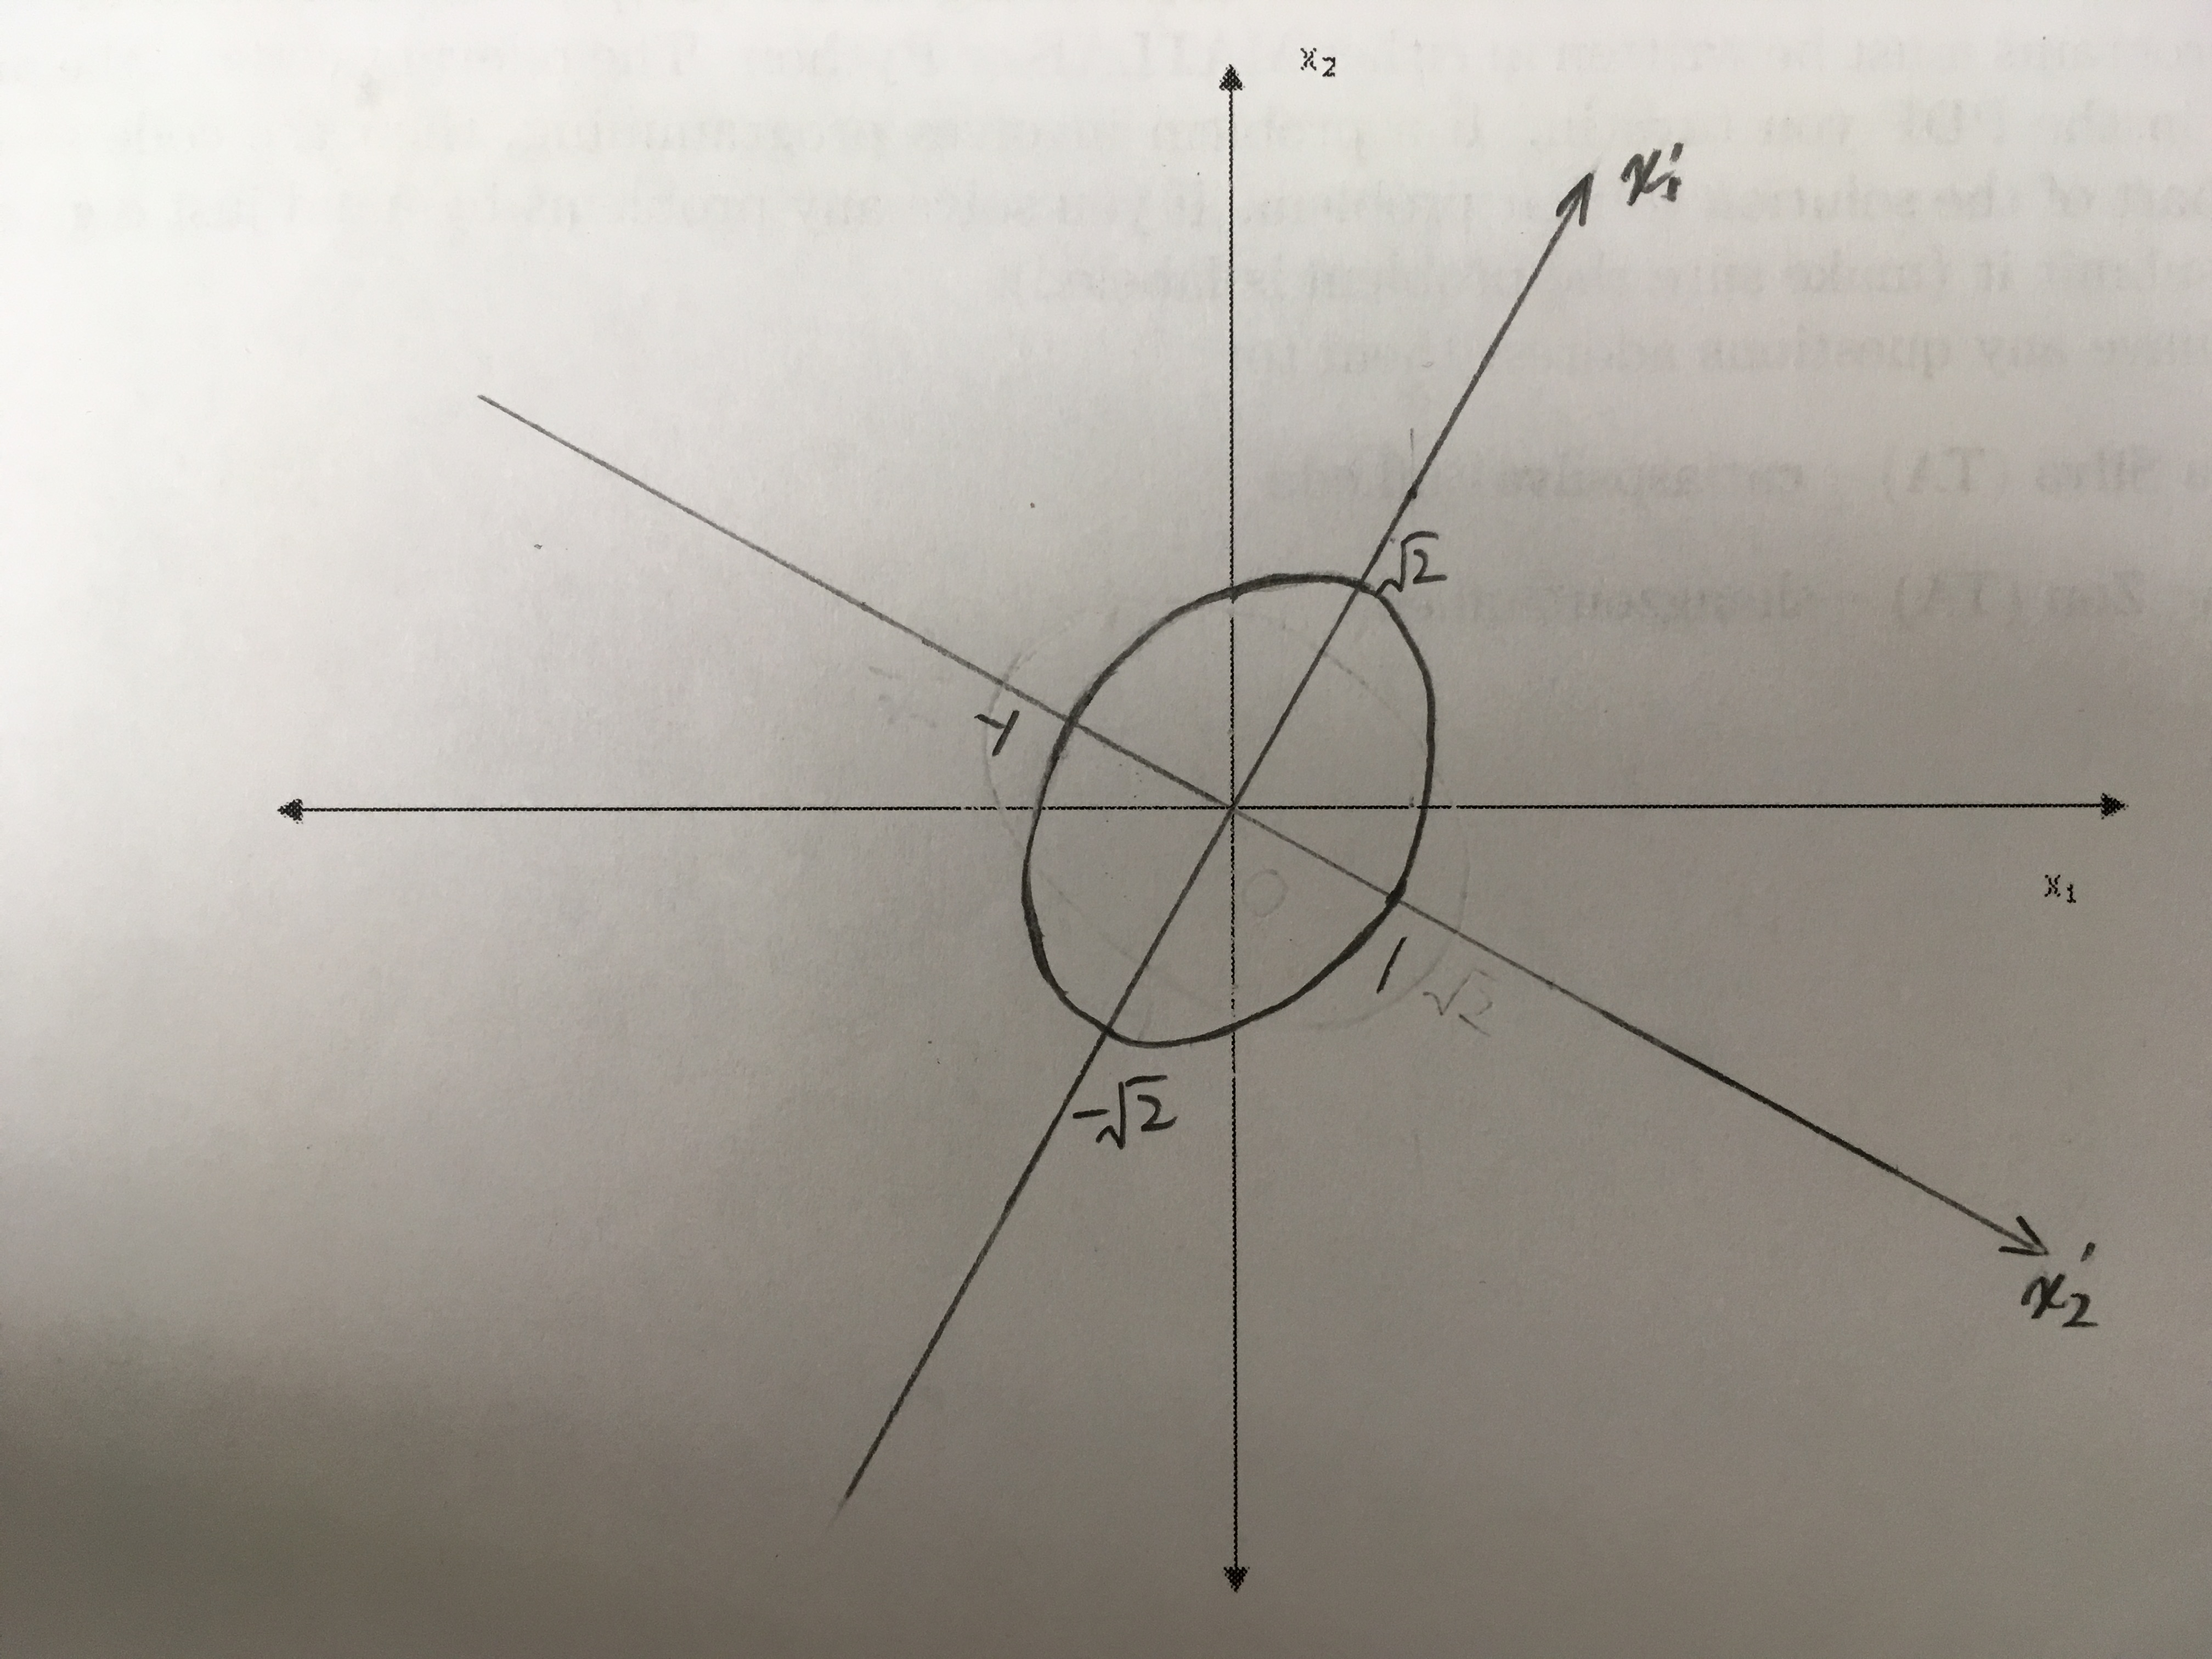
\includegraphics[width=3.5in]{1.jpeg}
	        \caption{New coordinate system and the curve describing all points with a Mahalanobis distance of 1 from the origin}
	        \label{fig:side:a}
	  \end{figure}
	

	
\section*{\huge\textbf{ Question 2} }	\large{Solution:\\}
	\normalsize
	If matrix A is eigendecomposible, which means matrix A is a diagonalizable $n\times n$ square matrix with $n$ eigenvalues $\lambda_1$,  $			\lambda_2$, ...  $\lambda_n$ and corresponding normalized eigenvectors $\mathbf{e_1}$,  $\mathbf{e_2}$, ...  $\mathbf{e_n}$. We have
	$$\Lambda = PAP^T$$
	, where $P^T = \left[\begin{matrix} \mathbf{e_1} & \mathbf{e_2} & ...& \mathbf{e_n}\end{matrix}\right]$, $\Lambda$ is a diagonal matrix.\\
	$P^TP = \left[\begin{matrix} \mathbf{e_1} & \mathbf{e_2} & ... & \mathbf{e_n}\end{matrix}\right] \left[ \begin{matrix}  \mathbf{e_1}^T \\ \mathbf{e_2}^T 	\\ ... \\ \mathbf{e_n}^T\end{matrix}\right] = 1$, and $A = P^{-1}\Lambda(P^T)^{-1}$\\
	Let $Q = P^{-1}$, then $A = Q\Lambda Q^T$.\\
	$$A^k = (Q\Lambda Q^T)^k = Q\Lambda Q^T \times Q \Lambda Q^T \times ... \times Q\Lambda Q^T = Q\Lambda ^k Q^T$$
	, where $Q = P^{-1}$, P is 	defined by $P^T = \left[\begin{matrix} \mathbf{e_1} & \mathbf{e_2} & ...& \mathbf{e_n}\end{matrix}\right]$, $
	\mathbf{e_i}(i = 1, 2, ..., n)$ are n eigenvectors of matrix A. 


\section*{\huge\textbf{ Question 3} } \large{Solution:\\}
	\normalsize The code I used to import the 3 files of dataset into MATLAB shows as below:
	\begin{lstlisting}
	addpath('/Users/hudanyun.sheng/Google Drive/Me/201708Fall/EEL5840FundamentalMachineLearning/homework/homework2')
	load ('ellipsoids.txt');
	load ('spheres.txt');
	load ('swissroll.txt');
	\end{lstlisting}
	To consider $\mathbf{X}$ to be any one of the dataset, simply use
	\begin{lstlisting}
	X = swissroll;
	\end{lstlisting}
	or 
	\begin{lstlisting}
	X = spheres;
	\end{lstlisting}
	or
	\begin{lstlisting}
	X = ellipsoids;
	\end{lstlisting}
	
	\textbf{3.1} 
	The MATLAB code used to calculate the covariance of every data set is shown below:
	\begin{lstlisting}
	mu = mean(X);
	X_std = X - mu;
	cov_mat = cov(X_std);
	\end{lstlisting}
	 ``cov\_mat" is the desired covariance matrix. 
	 
	 \begin{enumerate}[-]
	 
	 \item
	 For the \textbf{``Swiss Roll"} data set, the covariance matrix is 
	 $$\left[\begin{matrix} 43.2882 & 0.1535 & 4.4555 \\ 0.1535 & 10.5800 & 0.1544 \\ 4.4555 & 0.1544 & 47.1548 \end{matrix}\right]$$
	 
	 \item
	 For the \textbf{``Spheres"} data set, the covariance matrix is
	 $$\left[\begin{matrix} 10.0368 & 8.9743 & 9.0941 \\ 8.9743 & 9.9246 & 9.0678 \\ 9.0941 & 9.0678 & 10.2626 \end{matrix}\right]$$
	 
	 \item
	  For the \textbf{``Ellipsoids"} data set, the covariance matrix is
	 $$\left[\begin{matrix} 57.8661 & 14.6934 & 7.3664 \\ 14.6934 & 9.8630 & 4.5264 \\ 7.3664 & 4.5264 & 3.3570 \end{matrix}\right]$$
	\end{enumerate}
	
	\textbf{3.2}  
	The MATLAB code used to find the eigenvectors and eigenvalues of the covariance matrix is shown below:
	\begin{lstlisting}
	[eigenVecs, eigenVals] = eig(cov_mat);
	\end{lstlisting}
	``eigenVals" is the diagonal matrix with eigenvalues of covariance matrix at the diagonal, ``eigenVecs" a matrix whose columns are the         		corresponding eigenvectors.
	\begin{enumerate}[-]
	
	\item
	For the \textbf{``Swiss Roll"} data set, the eigenvalues of the covariance matrix are $\lambda_1 = 10.5788$, $\lambda_2 = 40.3647$, $\lambda_3 = 	50.0795$, and the corresponding eigenvectors of the covariance matrix are\\
	
	 $\mathbf{e_1} = \left[\begin{matrix} 0.0042 \\ -1.0000 \\ 0.0037\end{matrix}\right]$, 
	 $\mathbf{e_2} = \left[\begin{matrix} 0.8361 \\ 0.0015 \\ -0.5486\end{matrix}\right]$, 
	 and $\mathbf{e_3} = \left[\begin{matrix} 0.5486 \\ 0.0054 \\ 0.8361\end{matrix}\right]$.\\
	 
	\item
	For the \textbf{``Spheres"} data set, the eigenvalues of the covariance matrix are $\lambda_1 = 1.0001$, $\lambda_2 = 1.0571$, $\lambda_3 = 	28.1668$, and the corresponding eigenvectors of the covariance matrix are\\
	
	$\mathbf{e_1} = \left[\begin{matrix} 0.5318 \\ -0.8043 \\  0.2652\end{matrix}\right]$, 
	$\mathbf{e_2} = \left[\begin{matrix} 0.6207 \\ 0.1572 \\ -0.7681\end{matrix}\right]$, 
	and $\mathbf{e_3} = \left[\begin{matrix} 0.5760 \\ 0.5731 \\ 0.5829\end{matrix}\right]$.\\
	
	\item
	For the \textbf{``Ellipsoids"} data set, the eigenvalues of the covariance matrix are $\lambda_1 = 1.0352$, $\lambda_2 = 6.8856$, $\lambda_3 = 	6
	3.1653$, and the corresponding eigenvectors of the covariance matrix are\\ 
	
	$\mathbf{e_1} = \left[\begin{matrix} 0.0046\\ -0.4623\\ 0.8867\end{matrix}\right]$,
	$\mathbf{e_2} = \left[\begin{matrix} -0.3068\\ 0.8433\\ 0.4413\end{matrix}\right]$, 
	and $\mathbf{e_3} = \left[\begin{matrix} -0.9518\\ -0.2741\\ -0.1380\end{matrix}\right]$.\\
	\end{enumerate}
	
	\textbf{3.3} 
	The MATLAB code used to find and plot the projection of the data points into the 2-D and 1-D principal  
	components is shown below:
	\begin{lstlisting}
	w2 = eigenVecs(:,2:3);
	w1 = eigenVecs(:,3);
	X_pca2 = X_std * w2;
	X_pca1 = X_std * w1;
	figure
	scatter(X_pca2(:,1), X_pca2(:,2))
	xlabel('pc1', 'FontSize', 12, 'FontWeight', 'bold');
	ylabel('pc2', 'FontSize', 12, 'FontWeight', 'bold')
	title('Swiss Roll into 2-D', 'FontSize', 20, 'FontWeight', 'bold');
	% title('Spheres into 2-D', 'FontSize', 20, 'FontWeight', 'bold');
	% title('Ellipsoids into 2-D', 'FontSize', 20, 'FontWeight', 'bold');
	figure
	scatter(X_pca1, zeros(size(X_pca1)))
	xlabel('pc', 'FontSize', 12, 'FontWeight', 'bold');
	title('Swiss Roll into 1-D', 'FontSize', 20, 'FontWeight', 'bold');
	% title('Spheres into 2-D', 'FontSize', 20, 'FontWeight', 'bold');
	% title('Ellipsoids into 2-D', 'FontSize', 20, 'FontWeight', 'bold');
	\end{lstlisting}
	
	 \begin{enumerate}[-]
	 \newpage
	\item The \textbf{``Swiss Roll"} dataset:
	  \begin{figure}[H]
	    \begin{minipage}[t]{0.5\textwidth}
	        \centering
	        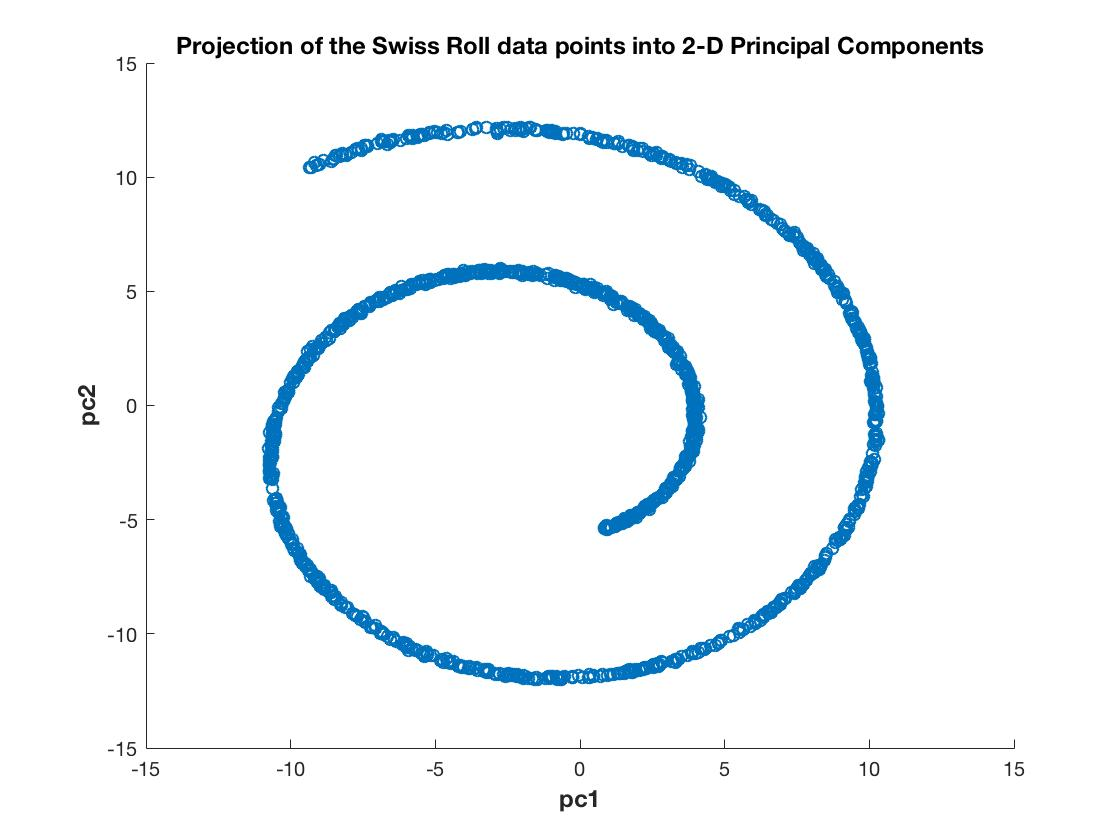
\includegraphics[width=4in]{1_1.jpg}
	        \caption{projection of ``Swiss Roll" into the 2-D}
	        \label{fig:side:a}
	    \end{minipage}%
	  \begin{minipage}[t]{0.5\textwidth}
	      \centering
	      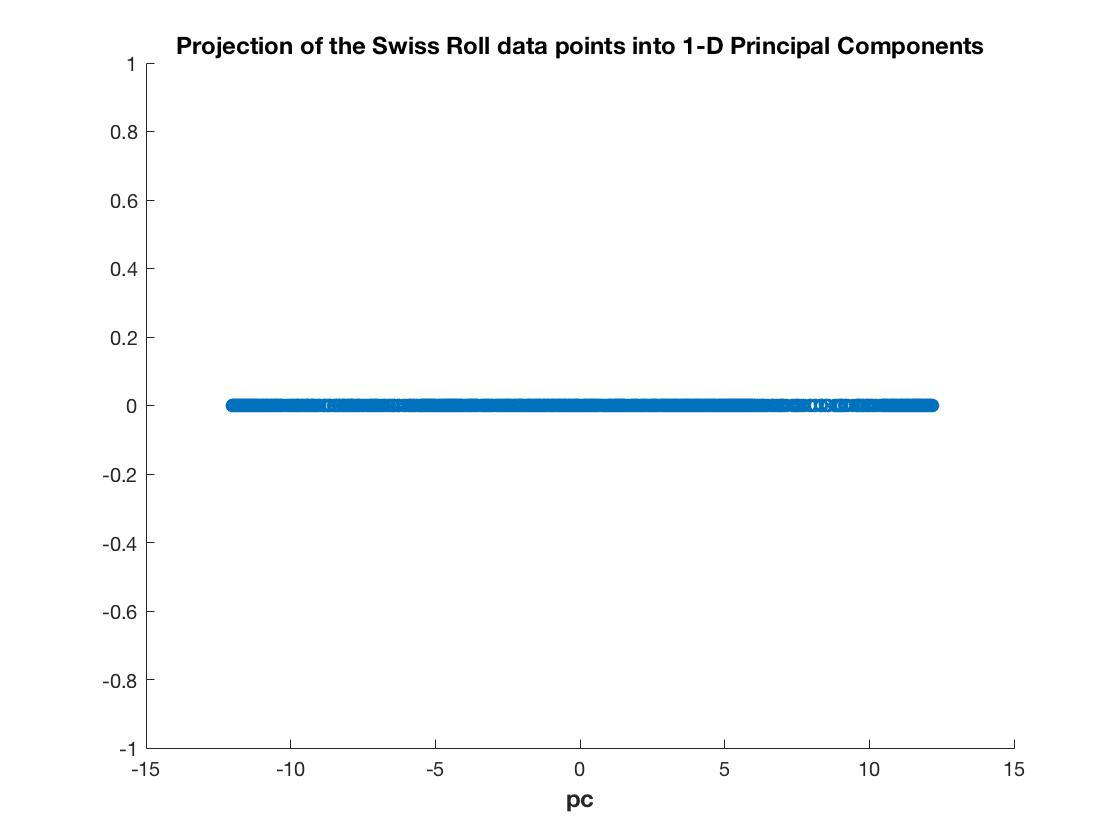
\includegraphics[width=4in]{1_2.jpg}
	      \caption{projection of ``Swiss Roll" into the 1-D}
	      \label{fig:side:b}
	    \end{minipage}
	  \end{figure}
	  
	  \begin{figure}[H]
	      \centering
	      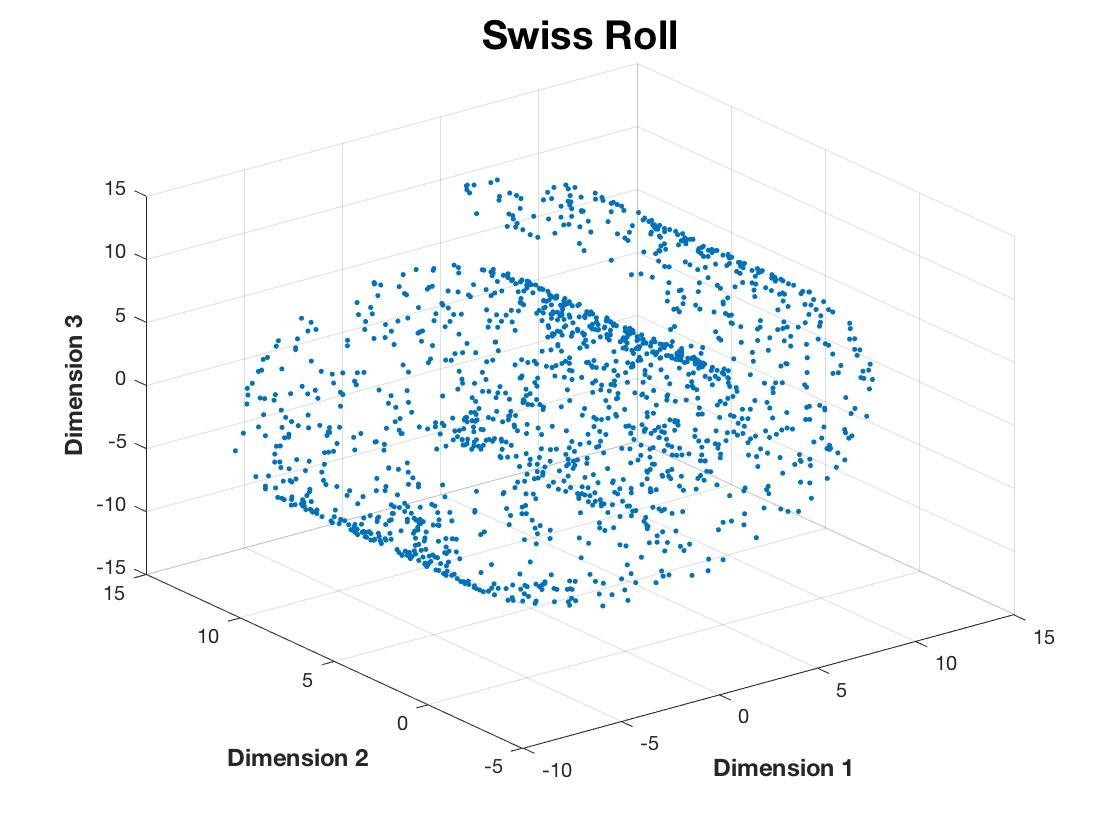
\includegraphics[width = 4.5in]{1_0.jpg}
	      \caption{original plot of the ``Swiss Roll" dataset}
	  \end{figure}
	  Based on the results, I would say that the 2-D projection preserve the most informative structure of the original data, while the 1-D projection has 
	  not the important information enough to represent the original dataset. For this ``Swiss Roll" dataset,  
\newpage	
	\item The \textbf{``Spheres"} dataset:
	 \begin{figure}[H]
	    \begin{minipage}[t]{0.5\textwidth}
	        \centering
	        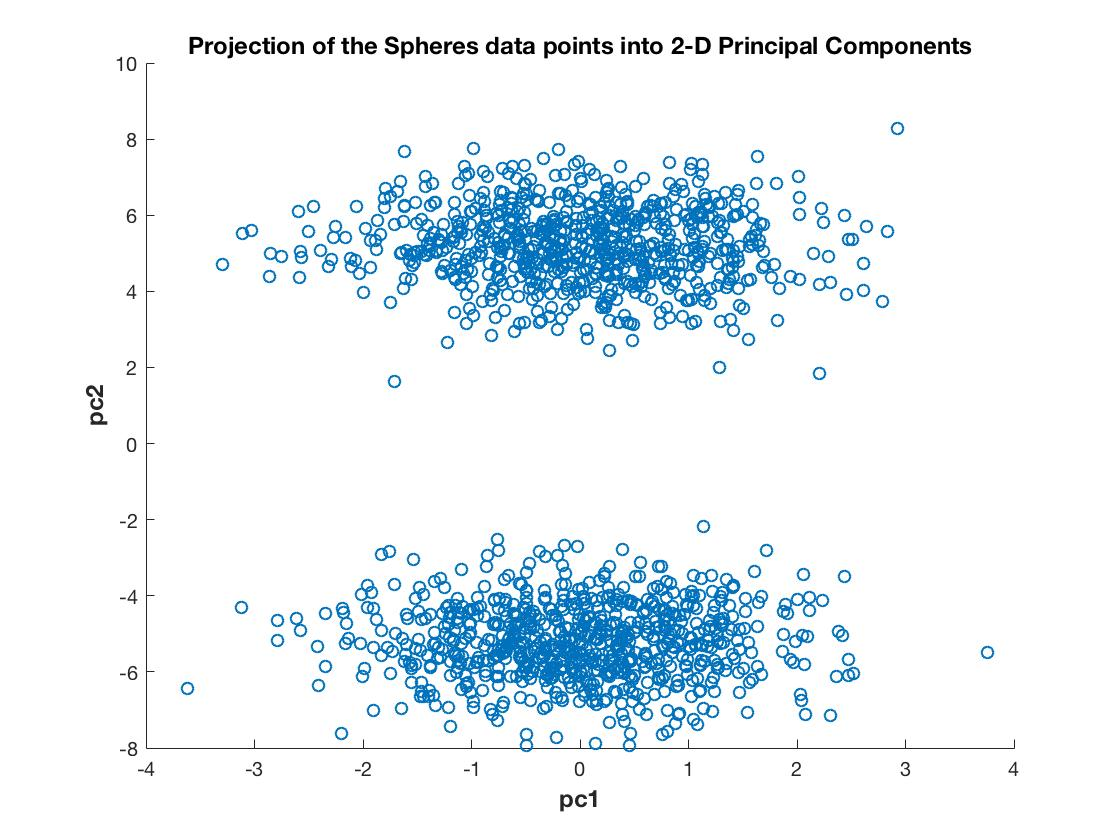
\includegraphics[width=4in]{2_2.jpg}
	        \caption{projection of ``Spheres" into the 2-D}
	        \label{fig:side:a}
	    \end{minipage}%
	  \begin{minipage}[t]{0.5\textwidth}
	      \centering
	      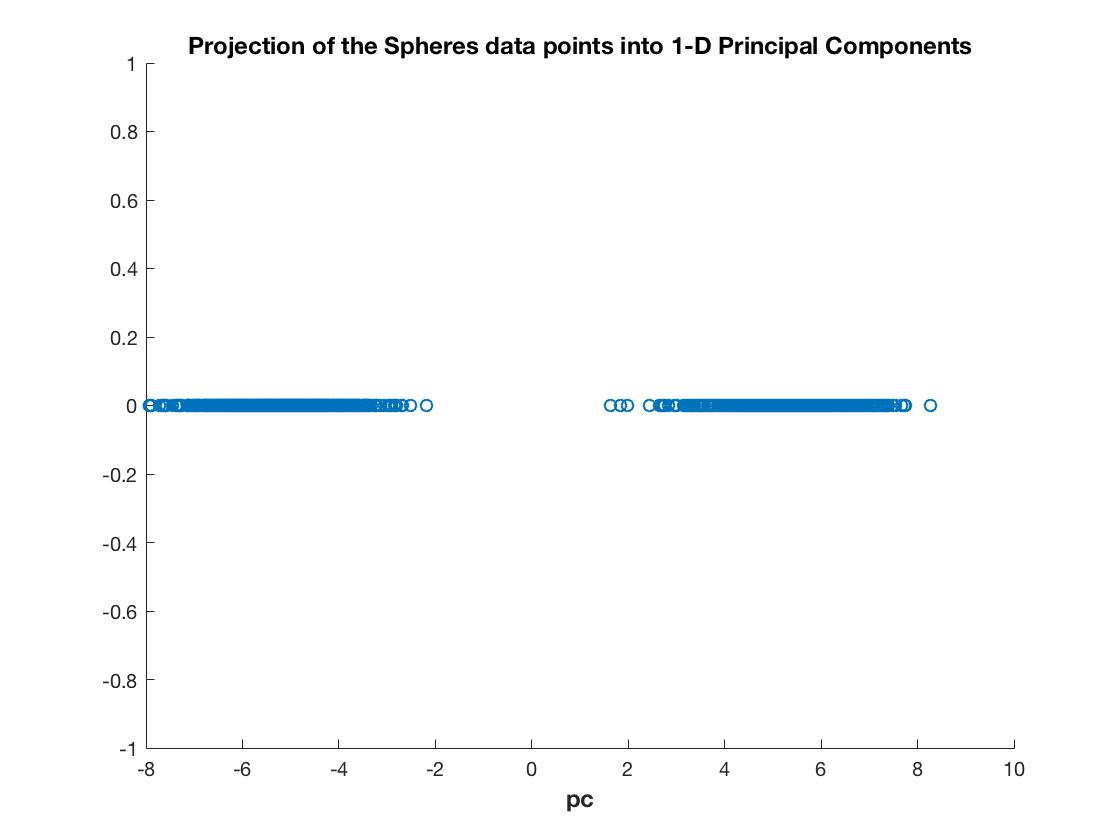
\includegraphics[width=4in]{2_1.jpg}
	      \caption{projection of ``Spheres" into the 1-D}
	      \label{fig:side:b}
	    \end{minipage}
	  \end{figure}
	  
	\begin{figure}[H]
	      \centering
	      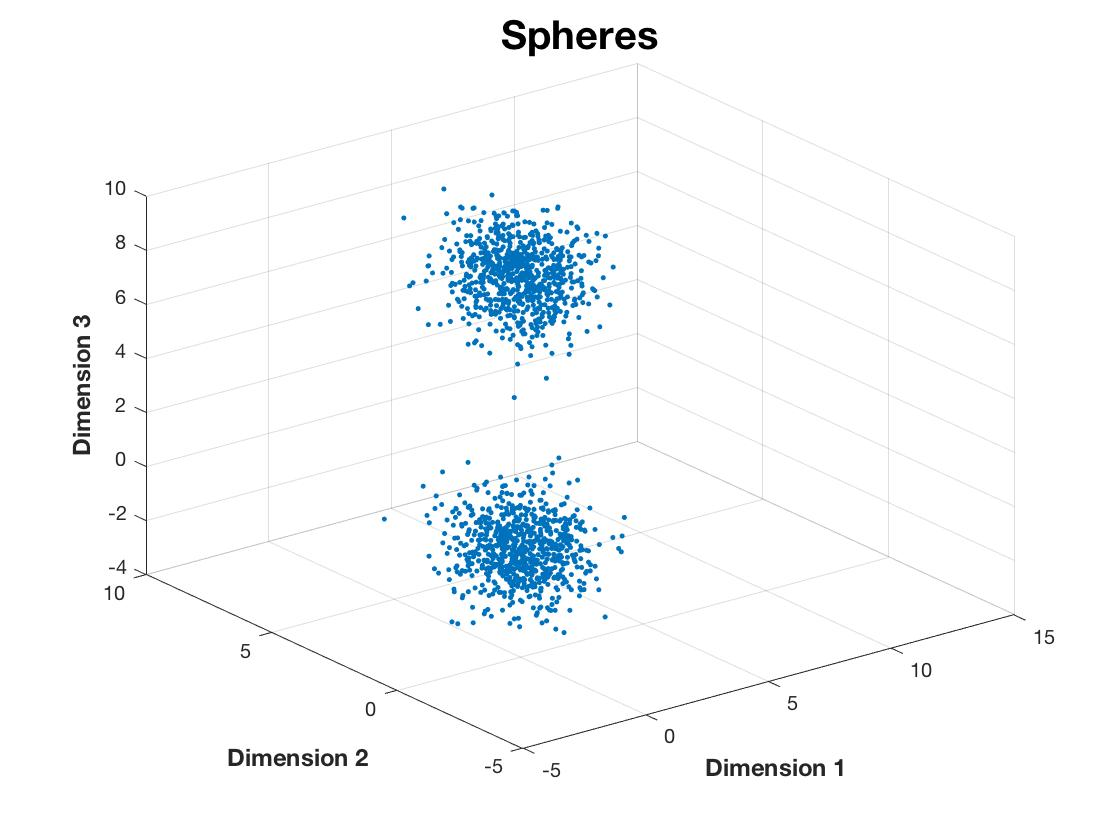
\includegraphics[width = 4.5in]{2_0.jpg}
	      \caption{original plot of the ``Spheres" dataset}
	  \end{figure}
	Based on the results, I would say that the 2-D projection preserve the most informative structure of the original data, while the 1-D projection has 
	not the important information enough to represent the original dataset. For this ``Spheres" dataset,  
\newpage
	\item The \textbf{``Ellipsoids"} dataset:
	\begin{figure}[H]
	    \begin{minipage}[t]{0.5\textwidth}
	        \centering
	        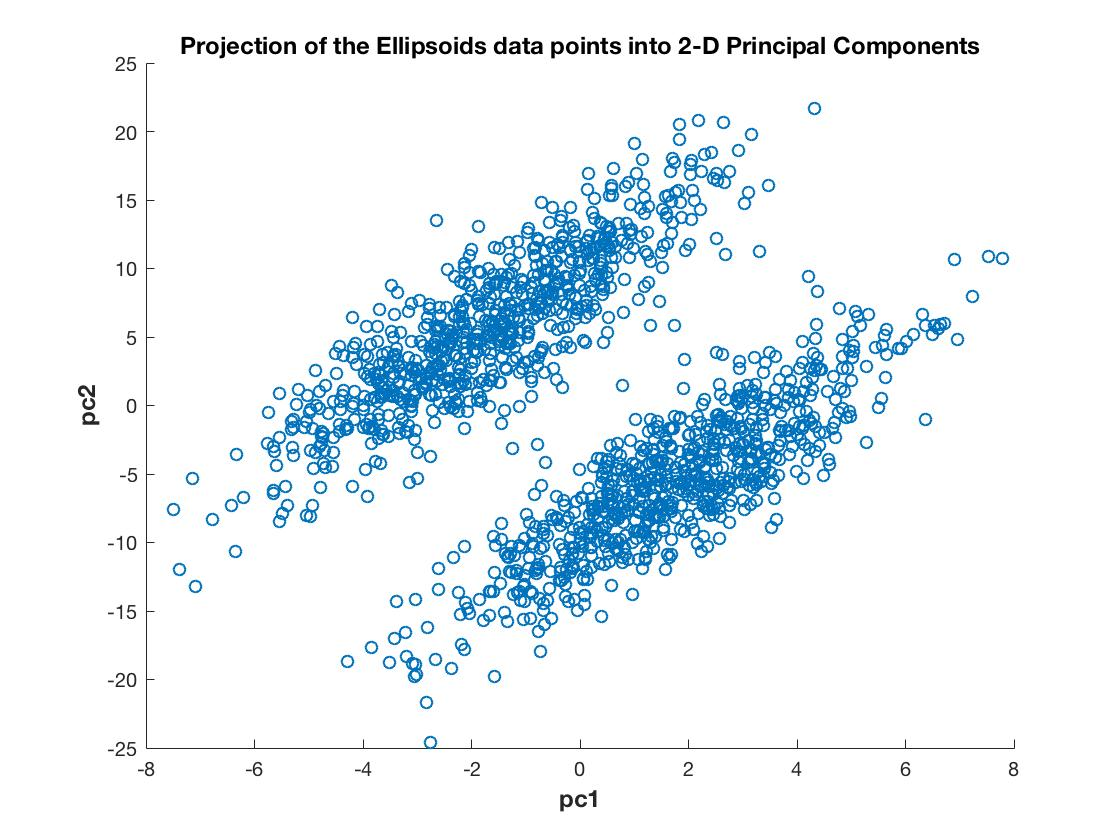
\includegraphics[width=4in]{3_2.jpg}
	        \caption{projection of ``Ellipsoids" into the 2-D}
	        \label{fig:side:a}
	    \end{minipage}%
	  \begin{minipage}[t]{0.5\textwidth}
	      \centering
	      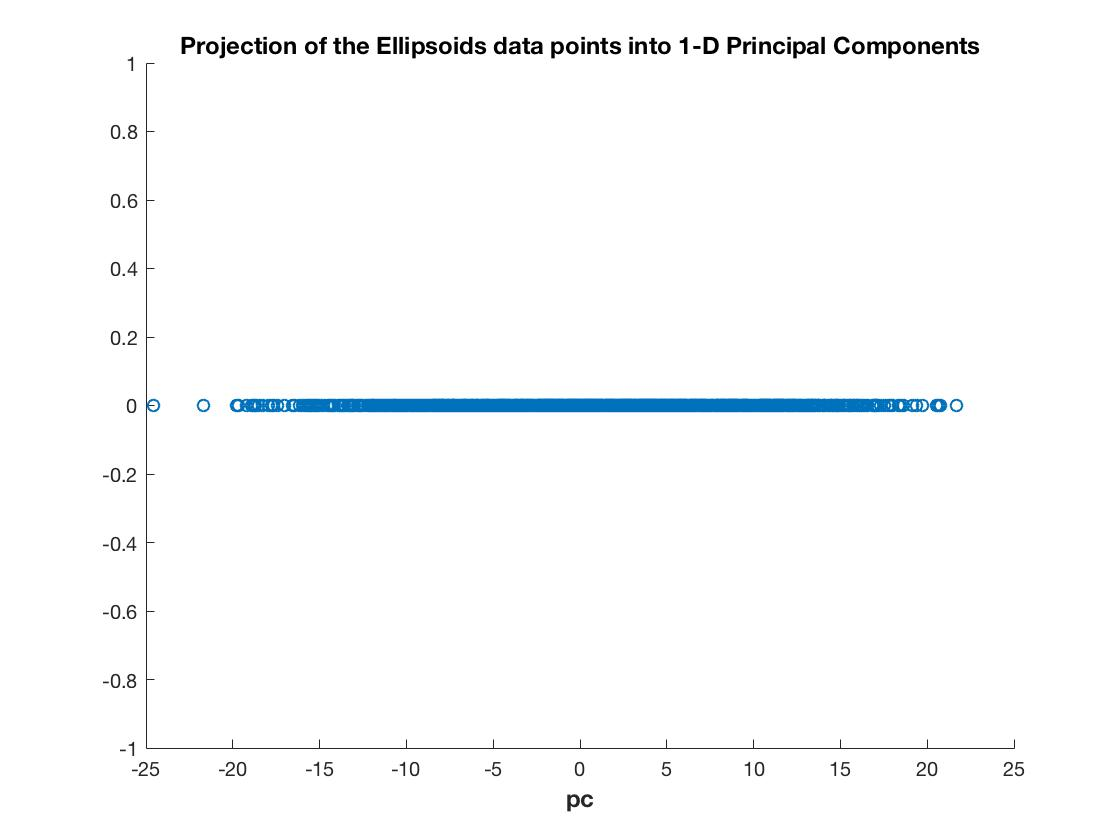
\includegraphics[width=4in]{3_1.jpg}
	      \caption{projection of ``Ellipsoids" into the 1-D}
	      \label{fig:side:b}
	    \end{minipage}
	  \end{figure}
	  
	\begin{figure}[H]
	      \centering
	      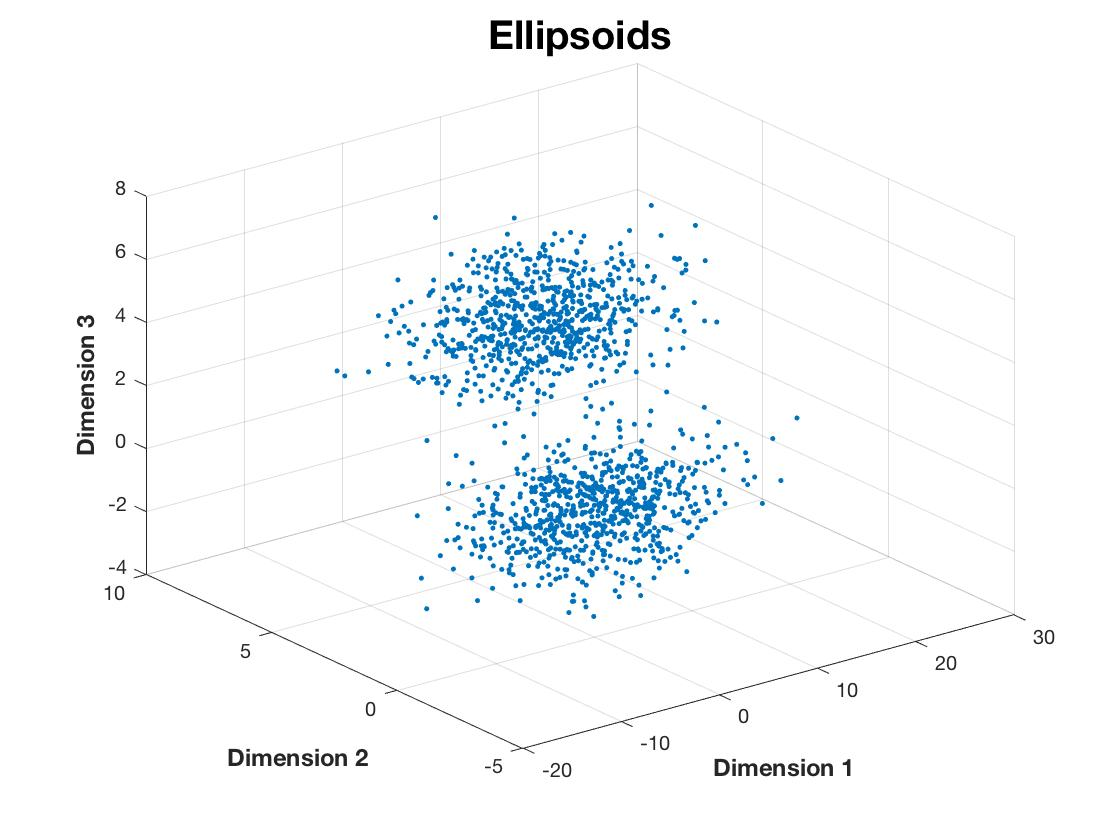
\includegraphics[width = 4.5in]{3_0.jpg}
	      \caption{original plot of the ``Swiss Roll" dataset}
	  \end{figure}
	Based on the results, I would say that the 2-D projection preserve the most informative structure of the original data, while the 1-D projection has not the important information enough to represent the original dataset. For this ``Ellipsoids" dataset,  
	 \end{enumerate}

	 
	
\end{spacing}
\end{document}